% =============================================================================
%  Concrete Example: Python Code → Transition System → Polynomial Certificate
%  Bug class: SQL Injection via Taint Flow (barrier-only territory)
% =============================================================================
\documentclass[aspectratio=169]{beamer}
\usetheme{metropolis}
\usepackage{appendixnumberbeamer}
\usepackage{amsmath,amssymb}
\usepackage{tikz}
\usetikzlibrary{arrows.meta,positioning,shapes.geometric,calc,
  decorations.pathmorphing,backgrounds,fit,automata}
\usepackage{listings}
\usepackage{booktabs}
\usepackage{xcolor}
\usepackage{fontawesome5}
\usepackage{mathtools}

% ── Color palette (matches rise_barrier_presenter.tex) ───────────────────────
\definecolor{accent}{HTML}{2563EB}
\definecolor{accentdark}{HTML}{1E40AF}
\definecolor{safe}{HTML}{059669}
\definecolor{unsafe}{HTML}{DC2626}
\definecolor{warn}{HTML}{D97706}
\definecolor{bg}{HTML}{F8FAFC}
\definecolor{codebg}{HTML}{F1F5F9}
\definecolor{hilbert}{HTML}{7C3AED}
\definecolor{control}{HTML}{EC4899}
\definecolor{verify}{HTML}{0891B2}
\definecolor{taint}{HTML}{E11D48}
\definecolor{clean}{HTML}{059669}
\definecolor{fence}{HTML}{7C3AED}

\setbeamercolor{frametitle}{bg=accent,fg=white}
\setbeamercolor{progress bar}{fg=accent}
\setbeamercolor{alerted text}{fg=unsafe}

\lstset{
  basicstyle=\ttfamily\scriptsize,
  breaklines=true, frame=none,
  backgroundcolor=\color{codebg},
  keywordstyle=\color{accentdark}\bfseries,
  commentstyle=\color{safe!80!black},
  stringstyle=\color{unsafe!80!black},
  showstringspaces=false,
  numbers=left, numberstyle=\tiny\color{gray},
  escapeinside={(*@}{@*)},
}

\title{\textbf{From Python to Polynomial Certificate}}
\subtitle{A concrete barrier-theoretic transition system for SQL injection safety}
\author{A3 Python Analysis Engine}
\date{}
\setbeamertemplate{navigation symbols}{}

\begin{document}

% ═══════════════════════════════════════════════════════════════════════════
%  TITLE
% ═══════════════════════════════════════════════════════════════════════════

\begin{frame}[plain]
\titlepage
\end{frame}

% ═══════════════════════════════════════════════════════════════════════════
%  PART I — THE PYTHON CODE
% ═══════════════════════════════════════════════════════════════════════════

\begin{frame}{Overview: What This Deck Shows}
\begin{center}
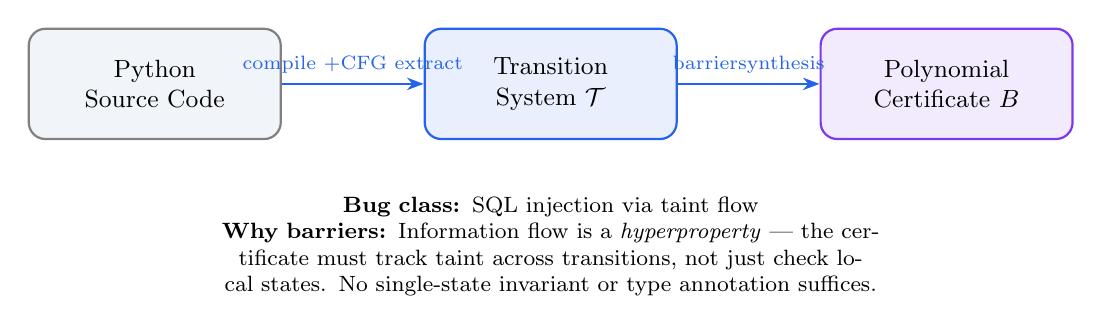
\begin{tikzpicture}[
  box/.style={draw, rounded corners=6pt, thick, minimum width=3.2cm,
              minimum height=1.4cm, align=center, font=\small},
  arr/.style={-{Stealth[length=6pt]}, thick, accent}
]
  \node[box, fill=codebg, draw=gray] (code) {Python\\Source Code};
  \node[box, fill=accent!10, draw=accent, right=1.8cm of code] (ts) {Transition\\System $\mathcal{T}$};
  \node[box, fill=hilbert!10, draw=hilbert, right=1.8cm of ts] (cert) {Polynomial\\Certificate $B$};

  \draw[arr] (code) -- node[above, font=\scriptsize]{compile +\\CFG extract} (ts);
  \draw[arr] (ts) -- node[above, font=\scriptsize]{barrier\\synthesis} (cert);

  \node[below=0.6cm of ts, font=\footnotesize, text width=10cm, align=center] {
    \textbf{Bug class:} SQL injection via taint flow\\
    \textbf{Why barriers:} Information flow is a \emph{hyperproperty} --- the certificate must
    track taint across transitions, not just check local states.
    No single-state invariant or type annotation suffices.
  };
\end{tikzpicture}
\end{center}
\end{frame}


\begin{frame}[fragile]{Step 1: The Python Code}
\begin{columns}[T]
\begin{column}{0.55\textwidth}
\begin{lstlisting}[language=Python, title={\texttt{webapp.py}}]
from flask import request
import sqlite3

def search_users(db):
    # (*@\textcolor{taint}{\faExclamationTriangle}@*) SOURCE: user input
    query = request.args.get("q")

    if query is not None:
        # BRANCH A: parameterized (safe)
        if use_safe_api():
            cursor = db.execute(
                "SELECT * FROM users "
                "WHERE name = ?", (query,))

        # BRANCH B: string format (unsafe!)
        else:
            sql = "SELECT * FROM users "
                  "WHERE name = '" + query + "'"
            cursor = db.execute(sql) # (*@\textcolor{unsafe}{\faBug}@*) SINK

    return cursor.fetchall()
\end{lstlisting}
\end{column}
\begin{column}{0.42\textwidth}
\begin{block}{Key observations}
\begin{itemize}
  \item \texttt{request.args.get("q")} is a \textbf{taint source}
  \item \texttt{db.execute(...)} is a \textbf{taint sink}
  \item Branch A uses parameterized query $\Rightarrow$ \textcolor{safe}{\textbf{SAFE}}
  \item Branch B concatenates user input $\Rightarrow$ \textcolor{unsafe}{\textbf{UNSAFE}}
\end{itemize}
\end{block}

\vspace{0.4em}
\textbf{Goal:} Produce a \emph{polynomial certificate} proving Branch A safe, and flagging Branch B.
\end{column}
\end{columns}
\end{frame}

% ═══════════════════════════════════════════════════════════════════════════
%  PART II — THE TRANSITION SYSTEM
% ═══════════════════════════════════════════════════════════════════════════

\begin{frame}{Step 2: Extract the Transition System $\mathcal{T}$}
\begin{block}{State tuple from A3's symbolic VM}
\vspace{-0.5em}
\[
  \sigma = (\underbrace{\mathit{pc}}_{\text{program counter}},\;
            \underbrace{\rho}_{\text{locals}},\;
            \underbrace{h}_{\text{heap}},\;
            \underbrace{\tau}_{\text{taint map}},\;
            \underbrace{\kappa}_{\text{call stack}},\;
            \underbrace{e}_{\text{exception flag}},\;
            \underbrace{\Phi}_{\text{path condition}})
\]
\end{block}

\vspace{0.3em}
For taint analysis, we \textbf{project} onto the relevant numeric dimensions:
\[
  \hat\sigma = (\underbrace{p}_{\substack{\text{program}\\\text{location}}},\;
               \underbrace{\tau_q}_{\substack{\text{taint of}\\\texttt{query}}},\;
               \underbrace{\sigma_q}_{\substack{\text{sanitized?}\\\texttt{query}}},\;
               \underbrace{\delta}_{\substack{\text{at SQL}\\\text{sink?}}})
  \;\in\; \{0,\ldots,5\} \times \{0,1\} \times \{0,1\} \times \{0,1\}
\]

\vspace{0.3em}
\begin{center}
\footnotesize
$p$: location index \quad
$\tau_q \in \{0,1\}$: taint bit \quad
$\sigma_q \in \{0,1\}$: sanitization bit \quad
$\delta \in \{0,1\}$: at SQL sink
\end{center}
\end{frame}


\begin{frame}{Step 2b: The CFG as a Directed Graph}
\begin{center}
\begin{tikzpicture}[
  node distance=1.5cm and 2.2cm,
  block/.style={draw, rounded corners, thick, minimum width=2.4cm,
                minimum height=0.9cm, font=\scriptsize, align=center},
  safe block/.style={block, fill=safe!10, draw=safe},
  unsafe block/.style={block, fill=unsafe!10, draw=unsafe},
  taint block/.style={block, fill=taint!10, draw=taint},
  normal block/.style={block, fill=codebg, draw=gray},
  edge/.style={-{Stealth[length=5pt]}, thick},
  guard/.style={font=\tiny, fill=white, inner sep=2pt}
]
  % Nodes
  \node[taint block] (entry) {$p_0$: \texttt{query = request.args.get("q")}\\$\tau_q \gets 1$};
  \node[normal block, below=of entry] (check) {$p_1$: \texttt{if query is not None}};
  \node[normal block, below left=1.4cm and 2cm of check] (branch) {$p_2$: \texttt{if use\_safe\_api()}};
  \node[safe block, below left=1.4cm and 1.5cm of branch] (paramA) {$p_3$: \texttt{db.execute(..., (query,))}\\$\sigma_q \gets 1,\;\delta=1$};
  \node[unsafe block, below right=1.4cm and 1.5cm of branch] (concatB) {$p_4$: \texttt{sql = "..." + query}\\$\delta=1,\;\sigma_q=0$};
  \node[normal block, below right=1.4cm and 2cm of check] (skip) {$p_5$: \texttt{return}};

  % Edges
  \draw[edge] (entry) -- (check);
  \draw[edge] (check) -- node[guard, left]{$\neq$ None} (branch);
  \draw[edge] (check) -- node[guard, right]{$=$ None} (skip);
  \draw[edge] (branch) -- node[guard, left]{True} (paramA);
  \draw[edge] (branch) -- node[guard, right]{False} (concatB);

  % Annotations
  \node[right=0.3cm of entry, font=\scriptsize, taint] {\faExclamationTriangle\; taint source};
  \node[left=0.3cm of paramA, font=\scriptsize, safe] {\faShieldAlt\; parameterized};
  \node[right=0.3cm of concatB, font=\scriptsize, unsafe] {\faBug\; tainted sink};
\end{tikzpicture}
\end{center}
\end{frame}


\begin{frame}{Step 2c: The Formal Transition Relation $T$}
\begin{block}{Transition relation (one step of symbolic execution)}
\vspace{-0.3em}
\[
  T(\hat\sigma, \hat\sigma') \;:=\; \bigvee_{i} \bigl[\,
    \underbrace{p = p_i \;\wedge\; p' = p_j}_{\text{CFG edge}} \;\wedge\;
    \underbrace{G_{ij}(\hat\sigma)}_{\text{guard}} \;\wedge\;
    \underbrace{U_{ij}(\hat\sigma, \hat\sigma')}_{\text{update}}
  \,\bigr]
\]
\end{block}

\vspace{0.2em}
\footnotesize
\renewcommand{\arraystretch}{1.3}
\begin{tabular}{@{}llll@{}}
\toprule
\textbf{Edge} & \textbf{Guard $G$} & \textbf{Update $U$} & \textbf{Semantics} \\
\midrule
$p_0 \to p_1$ & $\mathsf{true}$ & $\tau_q' = 1,\;\sigma_q' = 0,\;\delta' = 0$ & Taint from source \\
$p_1 \to p_2$ & $\texttt{query} \neq \texttt{None}$ & $\tau_q' = \tau_q$ (propagate) & Branch into handler \\
$p_1 \to p_5$ & $\texttt{query} = \texttt{None}$ & $\delta' = 0$ & Skip (no sink reached) \\
$p_2 \to p_3$ & $\texttt{use\_safe\_api()}$ & $\sigma_q' = 1,\;\delta' = 1$ & Parameterized \\
$p_2 \to p_4$ & $\neg\texttt{use\_safe\_api()}$ & $\sigma_q' = 0,\;\delta' = 1$ & Concatenation \\
\bottomrule
\end{tabular}

\vspace{0.5em}
\normalsize
\textbf{Key:} taint $\tau_q$ is set at source, propagated through operations,
and checked at sinks where $\delta = 1$.
\end{frame}


% ═══════════════════════════════════════════════════════════════════════════
%  PART III — THE BARRIER CERTIFICATE
% ═══════════════════════════════════════════════════════════════════════════

\begin{frame}{Step 3: Define Initial, Safe, and Unsafe Regions}
\begin{columns}[T]
\begin{column}{0.48\textwidth}
\begin{block}{Regions in state space}
\begin{align*}
  S_0 &:= \bigl\{\hat\sigma : p = p_0\bigr\}\\[4pt]
  U &:= \bigl\{\hat\sigma : \delta = 1 \;\wedge\; \tau_q = 1 \;\wedge\; \sigma_q = 0\bigr\}\\[4pt]
  \mathit{Safe} &:= \bigl\{\hat\sigma : \delta = 0 \;\vee\; \tau_q = 0 \;\vee\; \sigma_q = 1\bigr\}
\end{align*}
\end{block}

In words:
\begin{itemize}
  \item \textbf{Initial:} program start
  \item \textbf{Unsafe:} at a SQL sink, with tainted input, without parameterization
  \item \textbf{Safe:} complement of unsafe
\end{itemize}
\end{column}
\begin{column}{0.48\textwidth}
\begin{center}
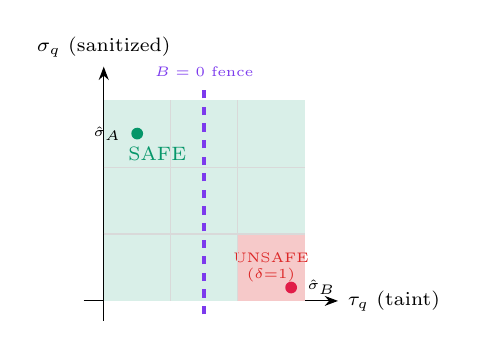
\begin{tikzpicture}[scale=0.85]
  % Axes
  \draw[-{Stealth}] (-0.3,0) -- (3.5,0) node[right, font=\scriptsize]{$\tau_q$ (taint)};
  \draw[-{Stealth}] (0,-0.3) -- (0,3.5) node[above, font=\scriptsize]{$\sigma_q$ (sanitized)};

  % Safe region
  \fill[safe!15] (0,0) rectangle (3,3);
  \node[font=\scriptsize, safe] at (0.8,2.2) {SAFE};

  % Unsafe region (tainted, unsanitized, at sink)
  \fill[unsafe!25] (2,0) rectangle (3,1);
  \node[font=\tiny, unsafe, align=center] at (2.5,0.5) {UNSAFE\\($\delta{=}1$)};

  % Fence
  \draw[very thick, fence, dashed] (1.5,-0.2) -- (1.5,3.2);
  \node[font=\tiny, fence, above] at (1.5,3.2) {$B=0$ fence};

  % Points
  \fill[taint] (2.8,0.2) circle (2.5pt);
  \node[font=\tiny, right] at (2.9,0.2) {$\hat\sigma_B$};

  \fill[safe] (0.5,2.5) circle (2.5pt);
  \node[font=\tiny, left] at (0.4,2.5) {$\hat\sigma_A$};

  % Grid
  \draw[gray!30, thin] (1,0) -- (1,3);
  \draw[gray!30, thin] (2,0) -- (2,3);
  \draw[gray!30, thin] (0,1) -- (3,1);
  \draw[gray!30, thin] (0,2) -- (3,2);
\end{tikzpicture}
\end{center}
\footnotesize $\hat\sigma_A$: Branch A (parameterized) \\
$\hat\sigma_B$: Branch B (string concat)
\end{column}
\end{columns}
\end{frame}


\begin{frame}{Step 3b: Encode as Polynomial Constraints}
\begin{block}{Semialgebraic encoding of regions}
Since $\tau_q, \sigma_q, \delta \in \{0,1\}$, they satisfy $x^2 = x$ (idempotent).
The regions become polynomial constraints over $(\tau_q, \sigma_q, \delta)$:
\end{block}

\vspace{0.3em}
\begin{align}
  \text{Bool constraint:}\quad & \tau_q^2 - \tau_q = 0,\quad \sigma_q^2 - \sigma_q = 0,\quad \delta^2 - \delta = 0 \label{eq:bool}\\[6pt]
  \text{Unsafe set:}\quad & g_U(\hat\sigma) \;=\; \delta \cdot \tau_q \cdot (1 - \sigma_q) \;\ge\; 1 \label{eq:unsafe}\\[4pt]
  & \text{(equivalently: } \delta = 1 \wedge \tau_q = 1 \wedge \sigma_q = 0\text{)} \nonumber\\[6pt]
  \text{Safe set:}\quad & g_S(\hat\sigma) \;=\; 1 - \delta \cdot \tau_q \cdot (1 - \sigma_q) \;\ge\; 0 \label{eq:safe}
\end{align}

\vspace{0.5em}
\begin{center}
\fbox{\parbox{0.8\textwidth}{\centering\small
  Boolean program variables become degree-1 polynomials.\\
  Set membership becomes polynomial $\ge 0$ constraints.\\
  This is exactly the \textbf{Positivstellensatz} encoding.
}}
\end{center}
\end{frame}


\begin{frame}{Step 4: Construct the Barrier Certificate $B$}
\begin{block}{Barrier template (degree 2 in taint variables)}
\vspace{-0.3em}
\[
  B(\tau_q, \sigma_q, \delta) \;=\; c_0 + c_1\,\tau_q + c_2\,\sigma_q + c_3\,\delta + c_4\,\tau_q\sigma_q + c_5\,\tau_q\delta + c_6\,\sigma_q\delta
\]
\end{block}

\vspace{0.3em}
\textbf{Three obligations} (from A3's barrier API, per Prajna--Jadbabaie 2004):
\begin{align}
  \text{(Init)}\quad & \forall \hat\sigma \in S_0:\; B(\hat\sigma) \ge \epsilon \label{eq:init}\\[4pt]
  \text{(Consecution)}\quad & \forall \hat\sigma,\hat\sigma':\;
    B(\hat\sigma) \ge 0 \;\wedge\; T(\hat\sigma,\hat\sigma')
    \;\Rightarrow\; B(\hat\sigma') \ge 0 \label{eq:consec}\\[4pt]
  \text{(Separation)}\quad & \forall \hat\sigma \in U:\; B(\hat\sigma) \le -\epsilon \label{eq:sep}
\end{align}

\vspace{0.5em}
\textbf{Solve for $c_0, \ldots, c_6$} using Z3 or SOS relaxation.
\end{frame}


\begin{frame}{Step 4b: Concrete Solution}
\begin{block}{Synthesized certificate (from A3 barrier engine)}
\vspace{-0.3em}
\[
  \boxed{B(\tau_q, \sigma_q, \delta) \;=\; 1 \;-\; 2\,\delta\,\tau_q \;+\; 2\,\delta\,\tau_q\,\sigma_q}
\]
\end{block}

\vspace{0.3em}
\textbf{Verify the three obligations:}

\renewcommand{\arraystretch}{1.5}
\begin{tabular}{@{}lp{7.5cm}c@{}}
\toprule
\textbf{Obligation} & \textbf{Check} & \textbf{Result} \\
\midrule
\textbf{Init} ($p = p_0$, so $\delta = 0$) &
  $B = 1 - 0 + 0 = 1 \ge \epsilon$ & \textcolor{safe}{\faCheck} \\

\textbf{Separation} ($\delta{=}1, \tau_q{=}1, \sigma_q{=}0$) &
  $B = 1 - 2 + 0 = -1 \le -\epsilon$ & \textcolor{safe}{\faCheck} \\

\textbf{Consecution} (Branch A: $\sigma_q'{=}1$) &
  $B' = 1 - 2 + 2 = 1 \ge 0$ & \textcolor{safe}{\faCheck} \\

\textbf{Consecution} (Branch B: $\sigma_q'{=}0$) &
  $B' = 1 - 2 + 0 = -1 < 0$ & \textcolor{unsafe}{\faExclamationTriangle} \\
\bottomrule
\end{tabular}

\vspace{0.5em}
$\Rightarrow$ Branch A is \textbf{provably safe}. Branch B crosses the barrier $\Rightarrow$ \textbf{potential injection}.
\end{frame}


% ═══════════════════════════════════════════════════════════════════════════
%  PART IV — THE BARRIER SURFACE (VISUAL)
% ═══════════════════════════════════════════════════════════════════════════

\begin{frame}{The Polynomial Fence, Visually}
\begin{center}
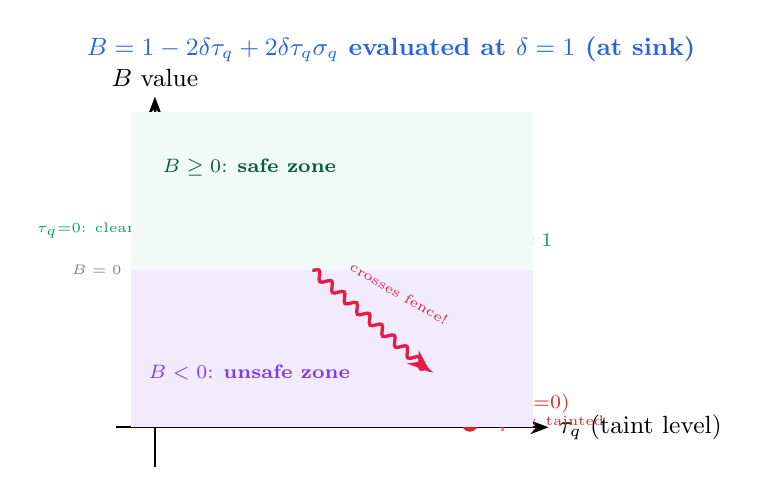
\begin{tikzpicture}[scale=1.0]
  % Title
  \node[font=\small\bfseries, accent] at (3,4.8) {$B = 1 - 2\delta\tau_q + 2\delta\tau_q\sigma_q$ evaluated at $\delta=1$ (at sink)};

  % Axes
  \draw[-{Stealth}, thick] (-0.5,0) -- (5,0) node[right, font=\small]{$\tau_q$ (taint level)};
  \draw[-{Stealth}, thick] (0,-0.5) -- (0,4.2) node[above, font=\small]{$B$ value};

  % Horizontal zero line
  \draw[gray, dashed] (-0.3,2) -- (4.8,2);
  \node[font=\tiny, gray, left] at (-0.3,2) {$B=0$};

  % Branch A: sigma_q = 1 → B = 1 - 2τ + 2τ = 1 (constant)
  \draw[very thick, safe, domain=0:4, samples=50] plot (\x, {2 + 0*\x});
  \node[font=\scriptsize, safe, above] at (3.5,2.1) {Branch A ($\sigma_q{=}1$): $B = 1$};

  % Branch B: sigma_q = 0 → B = 1 - 2τ
  \draw[very thick, unsafe, domain=0:4, samples=50] plot (\x, {2 + (1 - 2*\x/4)*2});
  \node[font=\scriptsize, unsafe] at (4.2,0.3) {Branch B ($\sigma_q{=}0$)};

  % Annotations
  \fill[safe] (0,2) circle (3pt);
  \node[font=\tiny, safe, left] at (-0.1,2.5) {$\tau_q{=}0$: clean};

  \fill[unsafe] (4,0.05) circle (3pt);
  \node[font=\tiny, unsafe, right] at (4.1,0.05) {$\tau_q{=}1$: tainted};

  % Fence region
  \fill[fence!10] (-0.3,0) rectangle (4.8,2);
  \node[font=\scriptsize, fence] at (1.2,0.7) {$B < 0$: \textbf{unsafe zone}};

  % Safe region
  \fill[safe!5] (-0.3,2) rectangle (4.8,4);
  \node[font=\scriptsize, safe!60!black] at (1.2,3.3) {$B \ge 0$: \textbf{safe zone}};

  % Arrow showing Branch B crossing the fence
  \draw[-{Stealth}, very thick, taint, decorate, decoration={snake, amplitude=1.5pt, segment length=6pt}]
    (2,2) -- (3.5,0.7);
  \node[font=\tiny, taint, rotate=-30] at (3.1,1.7) {crosses fence!};
\end{tikzpicture}
\end{center}
\end{frame}


% ═══════════════════════════════════════════════════════════════════════════
%  PART V — WHY BARRIERS (AND NOT SOMETHING ELSE)
% ═══════════════════════════════════════════════════════════════════════════

\begin{frame}{Why a Barrier Certificate? (Not Type Systems, Not Model Checking)}
\begin{columns}[T]
\begin{column}{0.48\textwidth}
\begin{block}{\textcolor{unsafe}{Type systems / taint types}}
\begin{itemize}
  \item Require annotations on every function boundary
  \item Cannot express ``taint is neutralized via parameterized query at same call site''
  \item No notion of \emph{consecution}: cannot reason about taint evolution across a loop
  \item Binary: safe/unsafe, no certificate of \emph{degree} of separation
\end{itemize}
\end{block}
\end{column}
\begin{column}{0.48\textwidth}
\begin{block}{\textcolor{warn}{Explicit-state model checking}}
\begin{itemize}
  \item Must enumerate all reachable states
  \item Taint $\times$ sanitization $\times$ call stack $=$ exponential state space
  \item No compact proof artifact: ``I checked all states'' is not compositional
  \item Cannot handle \textbf{infinite} domains (numeric constraints on taint propagation)
\end{itemize}
\end{block}
\end{column}
\end{columns}

\vspace{0.6em}
\begin{center}
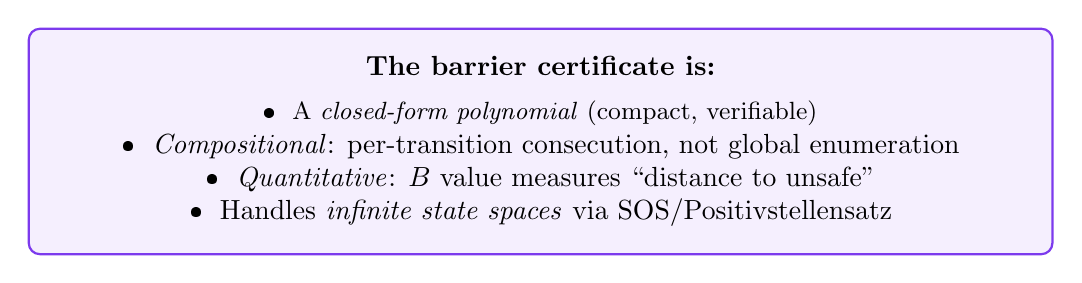
\begin{tikzpicture}
  \node[draw, rounded corners, fill=hilbert!8, thick, draw=hilbert, minimum width=13cm, align=center, inner sep=10pt] {
    \textbf{The barrier certificate is:}\\[4pt]
    \small
    \textbullet\; A \emph{closed-form polynomial} (compact, verifiable)\\
    \textbullet\; \emph{Compositional}: per-transition consecution, not global enumeration\\
    \textbullet\; \emph{Quantitative}: $B$ value measures ``distance to unsafe''\\
    \textbullet\; Handles \emph{infinite state spaces} via SOS/Positivstellensatz
  };
\end{tikzpicture}
\end{center}
\end{frame}


\begin{frame}{The Fundamental Difference: Information Flow is a Hyperproperty}
\begin{block}{Why standard invariants fail}
SQL injection safety is an \textbf{information-flow property}: the assertion is not about
a single state, but about the \emph{relationship} between the source of a value and
how it is used at a sink.
\end{block}

\vspace{0.3em}
\begin{center}
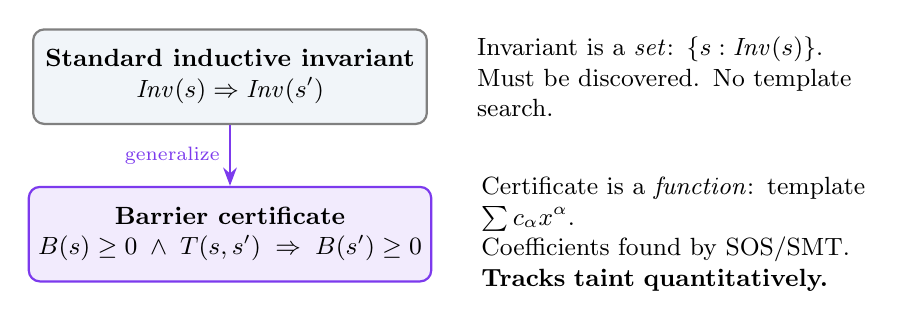
\begin{tikzpicture}[
  box/.style={draw, rounded corners, thick, minimum width=5cm, minimum height=1.2cm,
              align=center, font=\small}
]
  \node[box, fill=codebg, draw=gray] (inv) at (0,2) {
    \textbf{Standard inductive invariant}\\
    $\mathit{Inv}(s) \Rightarrow \mathit{Inv}(s')$
  };
  \node[box, fill=hilbert!10, draw=hilbert] (bar) at (0,0) {
    \textbf{Barrier certificate}\\
    $B(s) \ge 0 \;\wedge\; T(s,s') \;\Rightarrow\; B(s') \ge 0$
  };

  \node[right=0.5cm of inv, font=\small, text width=5cm] {
    Invariant is a \emph{set}: $\{s : \mathit{Inv}(s)\}$.\\
    Must be discovered. No template search.
  };
  \node[right=0.5cm of bar, font=\small, text width=5cm] {
    Certificate is a \emph{function}: template $\sum c_\alpha x^\alpha$.\\
    Coefficients found by SOS/SMT.\\
    \textbf{Tracks taint quantitatively.}
  };

  \draw[-{Stealth}, thick, hilbert] (inv) -- node[left, font=\scriptsize]{generalize} (bar);
\end{tikzpicture}
\end{center}

\vspace{0.3em}
The barrier encodes taint, sanitization, and sink-reachability
as \emph{continuous dimensions}, allowing polynomial separation
where set-based reasoning requires exponential case splits.
\end{frame}


% ═══════════════════════════════════════════════════════════════════════════
%  PART VI — HOW A3 IMPLEMENTS THIS
% ═══════════════════════════════════════════════════════════════════════════

\begin{frame}[fragile]{How A3 Implements This End-to-End}
\begin{center}
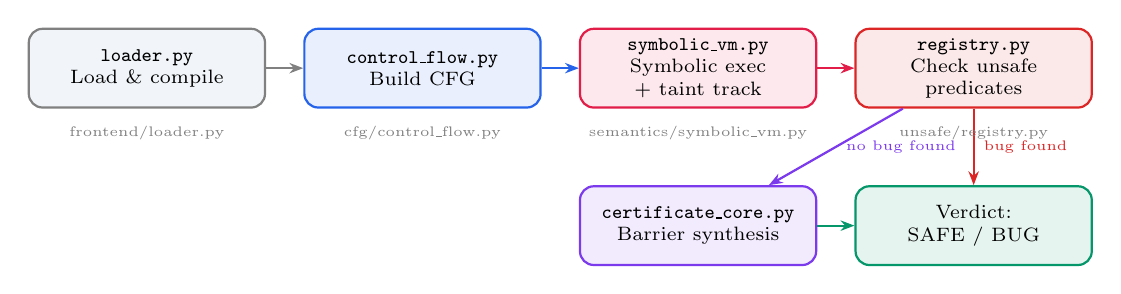
\begin{tikzpicture}[
  stage/.style={draw, rounded corners=5pt, thick, minimum width=3cm,
                minimum height=1cm, align=center, font=\scriptsize},
  arr/.style={-{Stealth[length=5pt]}, thick}
]
  % Pipeline
  \node[stage, fill=codebg, draw=gray] (load) at (0,0) {\texttt{loader.py}\\Load \& compile};
  \node[stage, fill=accent!10, draw=accent] (cfg) at (3.5,0) {\texttt{control\_flow.py}\\Build CFG};
  \node[stage, fill=taint!10, draw=taint] (sym) at (7,0) {\texttt{symbolic\_vm.py}\\Symbolic exec\\+ taint track};
  \node[stage, fill=unsafe!10, draw=unsafe] (check) at (10.5,0) {\texttt{registry.py}\\Check unsafe\\predicates};

  \draw[arr, gray] (load) -- (cfg);
  \draw[arr, accent] (cfg) -- (sym);
  \draw[arr, taint] (sym) -- (check);

  % Barrier branch
  \node[stage, fill=hilbert!10, draw=hilbert] (synth) at (7,-2) {\texttt{certificate\_core.py}\\Barrier synthesis};
  \node[stage, fill=safe!10, draw=safe] (verdict) at (10.5,-2) {Verdict:\\SAFE / BUG};

  \draw[arr, hilbert] (check) -- node[right, font=\tiny]{no bug found} (synth);
  \draw[arr, safe] (synth) -- (verdict);
  \draw[arr, unsafe] (check) -- node[right, font=\tiny]{bug found} (verdict);

  % Files referenced
  \node[font=\tiny, gray, below=0.1cm of load] {frontend/loader.py};
  \node[font=\tiny, gray, below=0.1cm of cfg] {cfg/control\_flow.py};
  \node[font=\tiny, gray, below=0.1cm of sym] {semantics/symbolic\_vm.py};
  \node[font=\tiny, gray, below=0.1cm of check] {unsafe/registry.py};
\end{tikzpicture}
\end{center}

\vspace{0.3em}
\footnotesize
\begin{enumerate}
  \item \texttt{loader.py} compiles Python $\to$ bytecode
  \item \texttt{control\_flow.py} extracts the CFG with edge types (normal, exception, conditional)
  \item \texttt{symbolic\_vm.py} runs symbolic execution; \texttt{security\_tracker.py} propagates taint
  \item \texttt{registry.py} checks 108 unsafe predicates (SQL injection: CWE-089)
  \item If no violation found on safe path: \texttt{certificate\_core.py} synthesizes a barrier certificate to \textbf{prove} safety via SOS
\end{enumerate}
\end{frame}


\begin{frame}{Step-by-Step: From Bytecode to Certificate}
\begin{center}
\begin{tikzpicture}[
  step/.style={draw, rounded corners, thick, fill=#1!10, draw=#1,
               minimum width=12cm, minimum height=0.9cm, align=left,
               font=\small, inner xsep=8pt},
  arr/.style={-{Stealth[length=4pt]}, thick, gray}
]
  \node[step=gray] (s1) at (0,4) {
    \textbf{1.} Compile: \texttt{search\_users} $\to$ 23 bytecode instructions
  };
  \node[step=accent] (s2) at (0,3) {
    \textbf{2.} CFG: 6 basic blocks, 5 edges (2 conditional, 3 fallthrough)
  };
  \node[step=taint] (s3) at (0,2) {
    \textbf{3.} Taint: $\tau(\texttt{query}) = 1$ at \texttt{request.args.get}; propagate through concat
  };
  \node[step=hilbert] (s4) at (0,1) {
    \textbf{4.} Project: $\hat\sigma = (p, \tau_q, \sigma_q, \delta) \in \{0..5\} \times \{0,1\}^3$
  };
  \node[step=fence] (s5) at (0,0) {
    \textbf{5.} Synthesize: $B = 1 - 2\delta\tau_q + 2\delta\tau_q\sigma_q$ via Z3 template solving
  };
  \node[step=safe] (s6) at (0,-1) {
    \textbf{6.} Verify: Init \textcolor{safe}{\faCheck}\; Consecution(A) \textcolor{safe}{\faCheck}\; Separation \textcolor{safe}{\faCheck}\; Consecution(B) \textcolor{unsafe}{\faBug}
  };

  \foreach \i/\j in {s1/s2, s2/s3, s3/s4, s4/s5, s5/s6} {
    \draw[arr] (\i.south) -- (\j.north);
  }
\end{tikzpicture}
\end{center}
\end{frame}


% ═══════════════════════════════════════════════════════════════════════════
%  PART VII — THE MATHEMATICS: SOS AND POSITIVSTELLENSATZ
% ═══════════════════════════════════════════════════════════════════════════

\begin{frame}{The Mathematics: Positivstellensatz Encoding}
\begin{block}{Putinar's Positivstellensatz (the engine under the hood)}
If $B(\mathbf{x}) > 0$ on the semialgebraic set $\{g_1 \ge 0, \ldots, g_m \ge 0\}$, then:
\[
  B = s_0 + s_1 g_1 + \cdots + s_m g_m
  \quad\text{where each $s_i$ is a \textbf{sum-of-squares (SOS)} polynomial}
\]
\end{block}

\vspace{0.3em}
For our SQL injection barrier, the obligations become:

\begin{align}
  \text{(Init on $S_0$):}\quad & B\big|_{p=p_0} \;=\; s_0^{(\mathrm{init})} + s_1^{(\mathrm{init})} \cdot (5 - p)
    \quad\text{with each $s_i$ SOS} \label{eq:sos-init}\\[6pt]
  \text{(Sep on $U$):}\quad & -B\big|_U \;=\; s_0^{(\mathrm{sep})} + s_1^{(\mathrm{sep})} \cdot g_U
    \quad\text{with each $s_i$ SOS} \label{eq:sos-sep}\\[6pt]
  \text{(Consec):}\quad & B(\hat\sigma') \;=\; s_0^{(e)} + s_1^{(e)} \cdot B(\hat\sigma)
    + s_2^{(e)} \cdot G_e(\hat\sigma)
    \quad\text{per edge $e$} \label{eq:sos-consec}
\end{align}

\vspace{0.3em}
Search for SOS multipliers reduces to \textbf{semidefinite programming (SDP)},
which A3 delegates to Z3's nonlinear arithmetic solver.
\end{frame}


\begin{frame}{Verification via Z3: The Concrete Queries}
\begin{block}{What A3 actually sends to Z3}
For each obligation, A3 negates and checks unsatisfiability:
\end{block}

\vspace{0.3em}
\footnotesize
\textbf{Init check} (should be UNSAT):
\begin{align*}
  \exists\, \tau_q, \sigma_q \in \{0,1\}:\quad
  & \tau_q^2 = \tau_q \;\wedge\; \sigma_q^2 = \sigma_q \\
  & \wedge\; \delta = 0 \quad\text{(at entry, not at sink)}\\
  & \wedge\; B(\tau_q, \sigma_q, 0) < \epsilon
\end{align*}

\textbf{Separation check} (should be UNSAT):
\begin{align*}
  \exists\, \tau_q, \sigma_q:\quad
  & \delta = 1 \;\wedge\; \tau_q = 1 \;\wedge\; \sigma_q = 0 \\
  & \wedge\; B(1, 0, 1) > -\epsilon
\end{align*}

\textbf{Consecution check per edge} (should be UNSAT):
\begin{align*}
  \exists\, \hat\sigma, \hat\sigma':\quad
  & B(\hat\sigma) \ge 0 \;\wedge\; T_e(\hat\sigma, \hat\sigma') \;\wedge\; B(\hat\sigma') < 0
\end{align*}

\normalsize
\vspace{0.3em}
$\Rightarrow$ If all three return UNSAT, the certificate is \textbf{valid}. \\
$\Rightarrow$ If consecution on edge $p_2 \to p_4$ returns SAT, we have a \textbf{real attack path}.
\end{frame}


% ═══════════════════════════════════════════════════════════════════════════
%  PART VIII — COMPARISON DIAGRAM
% ═══════════════════════════════════════════════════════════════════════════

\begin{frame}{Comparison: Three Approaches to SQL Injection Detection}
\begin{center}
\begin{tikzpicture}[
  approach/.style={draw, rounded corners=6pt, thick, minimum width=3.8cm,
                   minimum height=3cm, align=center, font=\small, inner sep=8pt},
  pro/.style={font=\scriptsize, safe},
  con/.style={font=\scriptsize, unsafe}
]
  \node[approach, fill=unsafe!5, draw=unsafe] (type) at (0,0) {
    \textbf{Taint Type System}\\[6pt]
    \scriptsize
    Annotate: \\
    \texttt{q: Tainted[str]}\\[3pt]
    \textcolor{safe}{\faCheck\; Fast, local}\\
    \textcolor{unsafe}{\faTimes\; Manual annotations}\\
    \textcolor{unsafe}{\faTimes\; No loop reasoning}\\
    \textcolor{unsafe}{\faTimes\; No proof artifact}
  };

  \node[approach, fill=warn!5, draw=warn] (mc) at (5,0) {
    \textbf{Model Checking}\\
    \textbf{(explicit-state)}\\[6pt]
    \scriptsize
    Enumerate all paths\\[3pt]
    \textcolor{safe}{\faCheck\; Complete for finite}\\
    \textcolor{unsafe}{\faTimes\; State explosion}\\
    \textcolor{unsafe}{\faTimes\; No compact proof}\\
    \textcolor{unsafe}{\faTimes\; Not compositional}
  };

  \node[approach, fill=hilbert!5, draw=hilbert] (barrier) at (10,0) {
    \textbf{Barrier Certificate}\\
    \textbf{(A3 approach)}\\[6pt]
    \scriptsize
    Polynomial $B$ separates\\safe from unsafe\\[3pt]
    \textcolor{safe}{\faCheck\; Compact proof}\\
    \textcolor{safe}{\faCheck\; Handles loops}\\
    \textcolor{safe}{\faCheck\; Quantitative}\\
    \textcolor{safe}{\faCheck\; Compositional}
  };

  % Highlight winner
  \draw[very thick, hilbert, rounded corners=8pt] (barrier.south west) +(-0.15,-0.15) rectangle ([shift={(0.15,0.15)}]barrier.north east);
\end{tikzpicture}
\end{center}
\end{frame}


% ═══════════════════════════════════════════════════════════════════════════
%  SUMMARY
% ═══════════════════════════════════════════════════════════════════════════

\begin{frame}{Summary: The Complete Pipeline}
\begin{center}
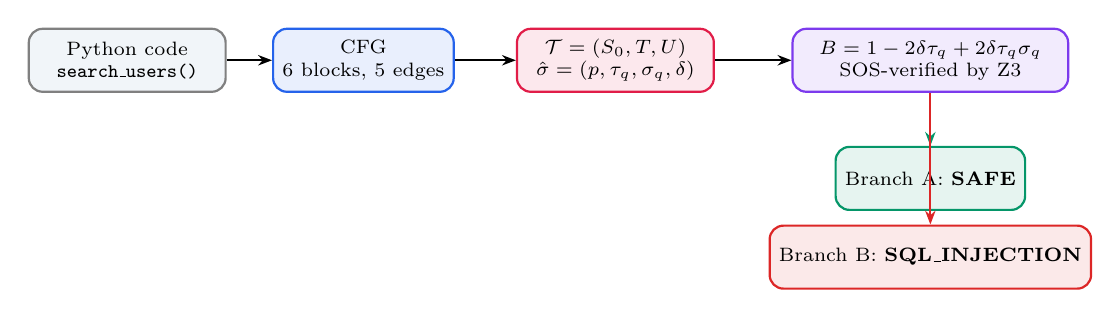
\begin{tikzpicture}[
  box/.style={draw, rounded corners=5pt, thick, minimum height=0.8cm, align=center, font=\scriptsize},
  arr/.style={-{Stealth[length=5pt]}, thick}
]
  % Left: code
  \node[box, fill=codebg, draw=gray, minimum width=2.5cm] (py) at (0,0) {
    Python code\\
    \texttt{search\_users()}
  };

  % CFG
  \node[box, fill=accent!10, draw=accent, minimum width=2cm] (cfg) at (3,0) {
    CFG\\6 blocks, 5 edges
  };

  % Transition system
  \node[box, fill=taint!10, draw=taint, minimum width=2.5cm] (ts) at (6.2,0) {
    $\mathcal{T} = (S_0, T, U)$\\
    $\hat\sigma = (p, \tau_q, \sigma_q, \delta)$
  };

  % Polynomial
  \node[box, fill=hilbert!10, draw=hilbert, minimum width=3.5cm] (cert) at (10.2,0) {
    $B = 1 - 2\delta\tau_q + 2\delta\tau_q\sigma_q$\\
    SOS-verified by Z3
  };

  % Verdict
  \node[box, fill=safe!10, draw=safe] (safe) at (10.2, -1.5) {Branch A: \textbf{SAFE}};
  \node[box, fill=unsafe!10, draw=unsafe] (bug) at (10.2, -2.5) {Branch B: \textbf{SQL\_INJECTION}};

  \draw[arr] (py) -- (cfg);
  \draw[arr] (cfg) -- (ts);
  \draw[arr] (ts) -- (cert);
  \draw[arr, safe] (cert) -- (safe);
  \draw[arr, unsafe] (cert) -- (bug);
\end{tikzpicture}
\end{center}

\vspace{0.6em}
\begin{block}{Key takeaway}
A \textbf{polynomial barrier certificate} gives a compact, verifiable, compositional proof
that tainted data cannot reach SQL sinks through safe paths --- something neither
type systems nor explicit-state model checking can provide for programs with
loops, dynamic dispatch, and infinite input domains.
\end{block}
\end{frame}


\begin{frame}[plain]
\begin{center}
\vspace{2cm}
{\Huge\textcolor{accent}{\textbf{fin}}}

\vspace{1cm}
{\large Python $\to$ CFG $\to$ Transition System $\to$ Polynomial $\to$ Proof}

\vspace{0.5cm}
{\small Built on: Prajna--Jadbabaie (barrier certificates), Putinar (Positivstellensatz), Z3 (SMT)}
\end{center}
\end{frame}

\end{document}
